\section{Problemstellung}
\label{sec:Problemstellung}

Bei der rheumatoiden Arthritis handelt es sich um eine Autoimmunerkrankung, bei der sich das Gelenkgewebe entzündet. Halten diese Entzündungen über längere Zeit an, werden die betroffenen Gelenke dadurch irreversibel geschädigt.

Die Erosion des Gelenkgewebes wird durch Fachpersonal anhand von Röntgenbildern eingestuft. Hierzu wird die Ratingen-Score verwendet, die das Fortschreiten der Erosion auf einer Skala von 0\% (gesundes Gelenk) bis bis 100\% (Gelenkgewebe vollständig erodiert) abbildet. Diese Einschätzung wurde bisher manuell vorgenommen, was pro Röntgenbild mehrere Minuten dauert. Dieser Vorgang wird als \textit{Scoring} bezeichnet.

Im Rahmen einer Bachelorarbeit an der ZHAW \cite{rohrbach2017} und in einem Folgeprojekt im Rahmen einer Masterarbeit (nicht öffentlich verfügbar) haben sich Janick Rohrbach (Zürcher Hochschule für Angewandte Wissenschaften), Tobias Reinhard (Seantis GmbH), Beate Sick (Universität Zürich) und Oliver Dürr (HTWG Konstanz) mit der Automatisierung des Scorings befasst \cite{rohrbach2019}. Dadurch soll der Vorgang einerseits beschleunigt werden, andererseits soll auch eine gleichbleibende Bewertungsqualität gewährleistet werden. Diese Verbesserungen dürften sich gerade bei umfassenden und langfristigen Studien als hilfreich erweisen.

Die automatische Auswertung von Bildern mit klassischen Machine-Learning-Metho\-den gestaltete sich bisher als schwierig. Mithilfe von \textit{Deep Convolutional Neuronal Networks}, die geeignete Merkmale von Bildern selbständig herausarbeiten, konnten auf diesem Gebiet in den letzten Jahren grosse Fortschritte erzielt werden.

Auf Basis von Röntgenbildern aus der SCQM\footnote{\url{https://www.scqm.ch/ueber-uns/} (abgerufen am 10.05.2020)}-Datenbank konnte ein entsprechendes Modell mit zehntausenden klassifizierten Gelenken trainiert, validiert und getestet werden. Hierbei stellte die Unausgeglichenheit der Testdaten ‒ ca. zwei Drittel der Röntgenbilder zeigen gesunde Gelenke ‒ eine grosse Herausforderung dar. Dennoch konnte ein Ergebnis erzielt werden, das sich sehen lässt: So stimmen die Bewertungen des automatischen Modells besser mit denjenigen von menschlichen Bewertungen überein, als die menschlichen Bewertungen untereinander.

Das Modell, bzw. die verschiedenen Modelle, die für den Scoring-Vorgang zum Einsatz kommen ‒ Erkennung von Körperteilen, Extraktion von Gelenken, Scoring von Gelenken ‒ beschränkt sich dabei auf linke Hände, bzw. auf zwei Arten von Gelenken: die Fingermittelgelenke zwischen dem ersten und zweiten Fingerglied jedes Fingers (proximale Interphalangealgelenke) und die Gelenke zwischen den Mittelhandknochen und dem ersten Fingerglied (Metacarpophalangealgelenke). Die Gelenke, jeweils von 1 (Daumen) bis 5 (kleiner Finger) nummeriert, sind auf \imgref{fig:xray-left-hand-annotated} eingezeichnet.

\begin{figure}
    \centering
    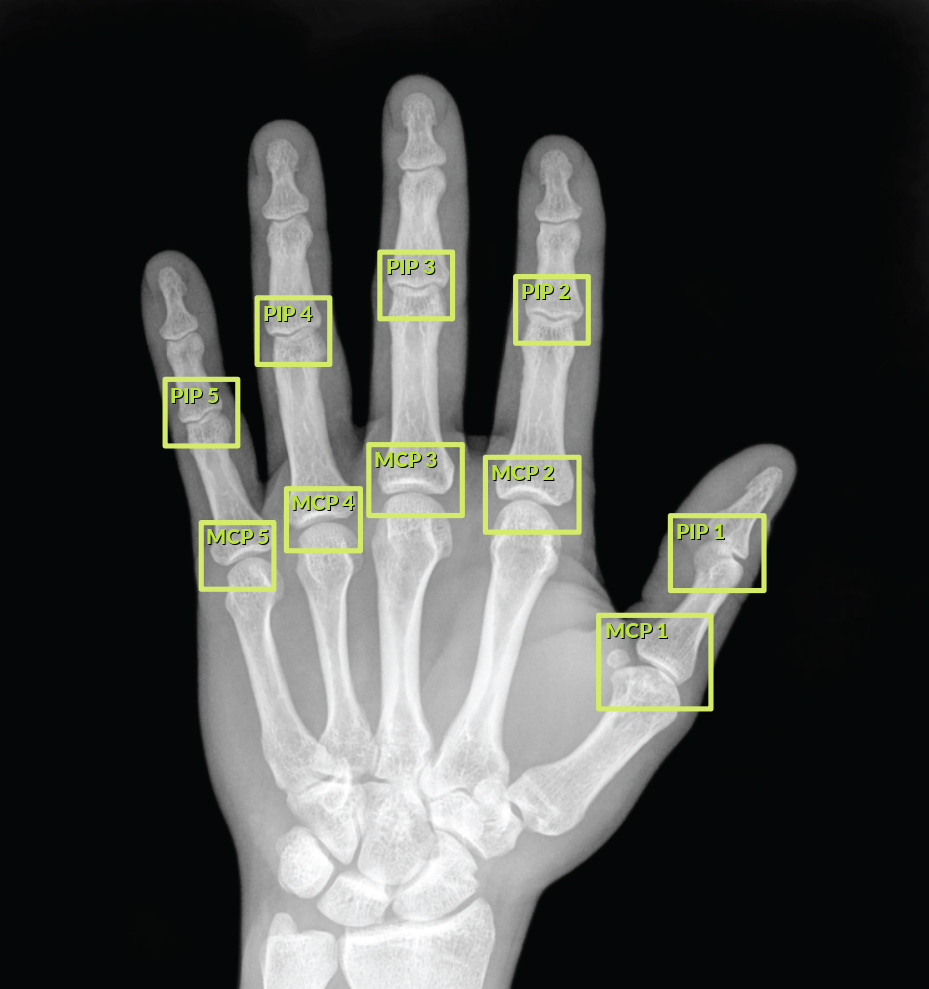
\includegraphics[width=\linewidth]{pics/xray-left-hand-annotated.png}
    \caption{Röntgenbild einer linken Hand mit markierten Metacarpophalangealgelenken (MCP) und proximalen Interphalangealgelenken (PIP), Quelle: \textit{OpenStax Anatomy and Physiology}, gefunden unter \url{https://commons.wikimedia.org/wiki/File:01_16_X-ray_of_Hand.jpg} (Lizenz: CC BY 4.0); Beschriftungen d.A.}
    \label{fig:xray-left-hand-annotated}
\end{figure}

Mit dem trainierten, validierten und erfolgreich getesteten Modell und dem dazu publizierten Fachartikel \textit{Bone Erosion Scoring for Rheumatoid Arthritis with Deep Convolutional Neural Networks}, \cite{rohrbach2019} ist der wissenschaftliche Grundstein für den produktiven Einsatz der automatischen Bewertung von Gelenken gemäss der Ratingen-Score gelegt. Bis dahin gibt es aber noch Einiges zu tun: Die erstellten Modelle müssen über einen Webservice zur Verfügung gestellt werden, damit sie in der Forschung zum Einsatz kommen können. Diese Aufgabe ist Gegenstand der vorliegenden Bachelorarbeit.

Geht es in der erwähnten Publikation \cite{rohrbach2019} v.a. um die Aspekte des Scorings im Bereich Machine Learning, liegt der Schwerpunkt in dieser Folgearbeit im Engineering-Bereich. Zunächst müssen die erstellten Modelle zu einer Software kombiniert werden, die als Web-Anwendung ansprechbar ist. Weiter muss sichergestellt werden, dass das automatische Scoring in nützlicher Frist durchgeführt werden kann ‒ gerade wenn das System unter hoher Last steht. Hierzu empfiehlt sich die Parallelisierung des Vorgangs: Die Röntgenbilder werden auf verschiedene Ausführungseinheiten verteilt. Dort wird das dargestellte Körperteil erkannt, es werden die relevanten Gelenke extrahiert und auf der Ratingen-Skala gescored. Am Schluss werden die ermittelten Scores als Gesamtergebnis zurückgeliefert.

Zudem sollen die Machine-Learning-Modelle austauschbar gemacht werden, sodass Verbesserungen auf diesem Gebiet schnell und einfach in den Produktivbetrieb einfliessen können. Hierbei ist es wichtig, dass die Qualität und Leistungsfähigkeit verschiedener Versionen miteinander verglichen werden können.

Das Ergebnis der Arbeit soll ein Prototyp für einen Webservice sein, der in bestehende Software eingebunden werden kann, um so ein automatisiertes, schnelles und präzises Scoring von Gelenken zu ermöglichen. Dadurch soll der Krankheitsverlauf von rheumatoider Arthritis besser nachverfolgt werden können, was etwa bei der Durchführung von Medikamentenstudien hilfreich sein kann.

\subsection{Projektauftrag}
\label{sec:projektauftrag}

Ziel der Arbeit ist es, den \textit{Proof of Concept}, der für die wissenschaftliche Publikation erstellt worden ist \cite{rohrbach2019}, für die Anwendung in der Praxis tauglich zu machen. Auf Basis der bestehenden Modelle, bzw. auf Basis des Codes zum Erstellen derselben, ist ein Deployment zu entwerfen und umzusetzen, das den Anforderungen des produktiven Betriebs genügt.

Die bestehenden Modelle sind in verschiedenen Versionen von TensorFlow umgesetzt worden. Zwar sollen die Modelle im Rahmen der vorliegenden Arbeit nicht auf eine aktuelle Version von TensorFlow migriert werden, es soll aber Teil der Arbeit sein, aufzuzeigen, was hierzu nötig wäre.

\subsubsection{Vorgaben}

Sämtliche Modelle, die für das Scoring eines Röntgenbildes benötigt werden, sind gegeben und vortrainiert. Sie erfüllen Minimum-Standars was ihre Performance betrifft.

\subsubsection{Erwartetes Resultat}
\label{sec:erwartetes-resultat}

Neben den für jede Bachelorarbeit zwingenden Resultate ‒ Schlussbericht (vorliegendes Dokument), Zwischen- und Schlusspräsentation, Web-Abstract, Einführungsvideo ‒ werden folgende Resultate vom Projekt erwartet:

\begin{enumerate}
    \item Stand der Technik zur Industrialisierung (Evaluation, Testing) von ML-Modellen
    \item Vorschlag für ein generisches Format von Modellen zum Exportieren aus ML-Frame\-works und zum Importieren zur Ausführung
    \item Vorschlag für geeignete Metriken zum Vergleich von Modellen
    \item Aufzeigen, was für eine Vereinheitlichung der Codebasis gemacht werden muss
    \item Lauffähiger Protoyp
    \begin{enumerate}
        \item Automatisierte Evaluation und Testing von neuen Modellen mit Vergleich zu alten Modellen und Minimum-Standards
        \item Visualisierung und Reporting der Performanz neuer Modelle
        \item API zum Ausführen des Modelles (Verteilen über mehrere GPUs)
        \item Load Balancing, Messaging Systems
        \item Nahtloses Austauschen von alten Modellen mit neuen Versionen
    \end{enumerate}
\end{enumerate}

\subsubsection{Abgrenzung}

Das Trainieren der Modelle ist nicht Teil der Arbeit. Die Modelle können als Blackbox betrachtet werden. Dementsprechend genügt es, sie aus einer High-Level-Sicht zu beschreiben.

Die effektive Integration in die Produktivumgebung von Seantis, sprich die Plattform \textit{HealthData.ai}\footnote{\url{https://www.healthdata.ai/en} (abgerufen am 27.05.2020)}, ist nicht Teil der Arbeit. Die hierzu notwendigen Schritte sollen jedoch beschrieben werden.

\subsection{Projektrisiken}
\label{sec:projektrisiken}

Im Folgenden werden verschiedene Projektrisiken und mögiche Mitigationsmassnahmen für diese aufgelistet:

\begin{description}
    \item[Keine lauffähigen Modelle] Die verschiedenen Modelle wurden teils vor mehreren Jahren entwickelt und trainiert. Ob sie tatsächlich funktionieren, und ob die Modelldaten noch in einem konsistenten Zustand auffindbar sind, ist zu Beginn des Projekts nicht klar.
        \begin{description}
            \item[Risiko] Eines oder mehrere Modelle sind nicht funktionstüchtig oder gar verloren.
            \item[Mitigation] Anhand von bestehendem Quellcode kann versucht werden, die Modelle neu zu erstellen. Scheitert dies, müssten fehlende Modelle durch Platzhalter (Mocks) ersetzt werden, die Predictions und ein bestimmtes Laufzeitverhalten simulieren.
        \end{description}
    \item[Aktualisierung der Modelle] Die zugrundeliegenden Modelle sind teils schon etwas älter und in unterschiedlichen Versionen bzw. mit unterschiedlichen Frameworks entwickelt worden.
        \begin{description}
            \item[Risiko] Die Modelle können nicht mit aktuellen Versionen der zugrundeliegenden Frameworks importiert werden.
            \item[Mitigation] Die Modelle werden mittels geeigneter Massnahmen (Container, virtuelle Umgebung) isoliert, sodass sie in ihrer ursprünglichen «Trainigsumgebung» ausgeführt werden können.
        \end{description}
    \item[Schlechte Performance (Prediction)] Da verschiedene Modelle zum Einsatz kommen, die bisher nie dem produktiven Betrieb ausgesetzt gewesen sind, kann es sein, dass deren Performance im Bezug auf die Qualität der Predictions schlecht ist.
        \begin{description}
            \item[Risiko] Eines oder mehrere Modelle weisen eine schlechte Prediction-Performance auf.
            \item[Mitigation] Dieses Risiko muss getragen werden. Die Prediction-Performance des Gesamtsystems ist durch das schwächste Modell nach oben begrenzt.
        \end{description}
    \item[Schlechte Performance (Laufzeit)] Für ein Scoring eines Röntgenbildes sind verschiedene Modelle in mehreren Schritten involviert.
        \begin{description}
            \item[Risiko] Die Laufzeit-Performance könnte so schwach ausfallen, dass ein produktiver Betrieb dadurch inpraktikabel wird.
            \item[Mitigation] Mit geeigneten architektonischen Massnahmen (parallele Abarbeitung, Ausführung auf GPUs) kann die Laufzeit-Performance erhöht werden. Genügt dies nicht, muss auf ein synchrones Ansprechen des Gesamtsystems zugunsten einer anderen, d.h. asynchronen Lösung verzichtet werden.
        \end{description}
    \item[Hoher Arbeitsspeicherverbrauch] Da mehrere Modelle für das Scoring eines Röntgenbildes benötigt werden, kann dies zu einem hohen Arbeitsspeicherverbrauch führen.
        \begin{description}
            \item[Risiko] Die Modelle und ihre umgebende Laufzeitumgebung können nicht gleichzeitig in den Arbeitsspeicher  eines Systems geladen werden.
            \item[Mitigation] Der Prototyp kann auf einem stärker bestückten System (etwa bei einem Cloud-Anbieter) ausgeführt oder über mehrere Systeme verteilt werden.
        \end{description}
\end{description}
